\section{Auswertung}
\label{sec:Auswertung}

Im folgenden werden die grundlegenden Eigenschaften des Ultraschalles, die in dem Versuch untersucht wurden, ausgewertet. \newline
Zunächst wurden die verwendeten Acrylplatten abgemessen. Die gemessenen Werte sind in der \autoref{tab:koerper} zu finden.

\begin{table}
  \centering
  \caption{Messwerte der Acrylplattten.}
  \label{tab:koerper}
  \begin{tabular}{c c}
    \toprule
    Platte $P_i$ & Dicke / $\si{\milli\meter}$ \\
    \midrule
    $P_1$ & 10 \\
    $P_2$ & 6 \\
    $\overline{P_i}$ & $8 \pm 2$ \\
    \bottomrule
  \end{tabular}
\end{table}

Die in \autoref{fig:reflexe} aufgenommene Grafik zeigt die vier Reflexe. Die Amplituden und Laufzeiten, die sich aus diesen Reflexen ergeben sind in \autoref{tab:refl}
eingetragen. Die Mittelwerte der Laufzeiten und der Amplituden sind ebenfalls in der Tabelle eingetragen.

\begin{figure}[H]
  \centering
  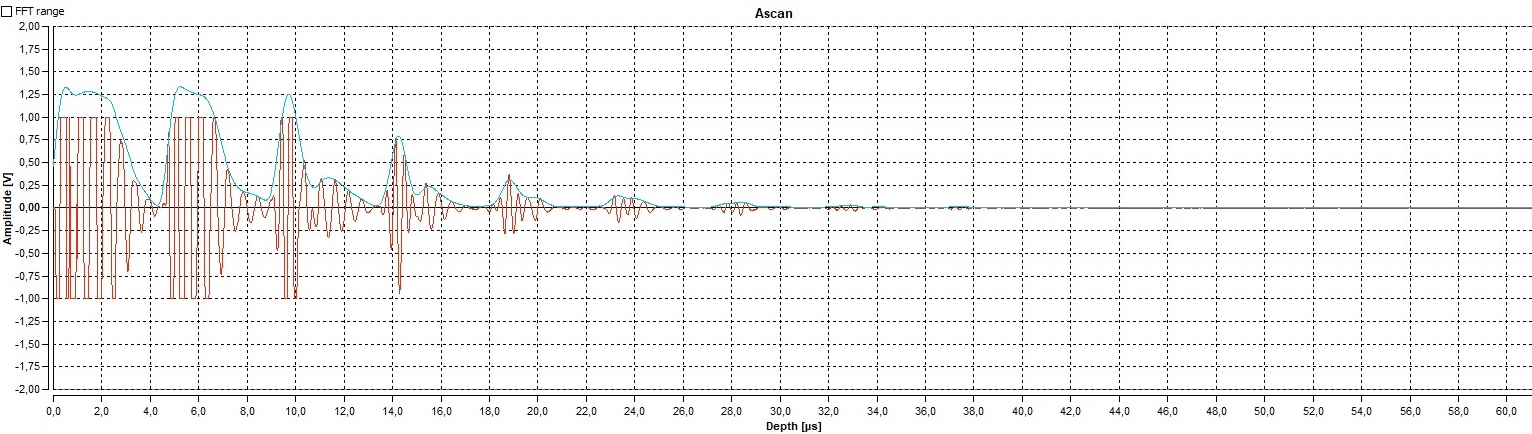
\includegraphics[width = \textwidth]{data/Geräteeinstellungen/reflexe.png}
  \caption{Aufgenommene Grafik zu den vier Reflexen.}
  \label{fig:reflexe}
\end{figure}

\begin{table}
  \centering
  \caption{Auswertung der aufgenommenen Grafik zu den vier Reflexen.}
  \label{tab:refl}
  \begin{tabular}{c c c}
    \toprule
    Reflex $R_i$ & Laufzeit / $\si{\micro\second}$ & Amplitude / $\si{\volt}$ \\
    \midrule
    $R_1$ & 4,0 & 1,30 \\
    $R_2$ & 4,9 & 1,30 \\
    $R_3$ & 4,8 & 1,25 \\
    $R_4$ & 3,2 & 0,80 \\
    $\overline R$ & $4.2 \pm 0.7$ & $1.16 \pm 0.21$ \\
    \bottomrule
  \end{tabular}
\end{table}

\begin{figure}[H]
  \centering
  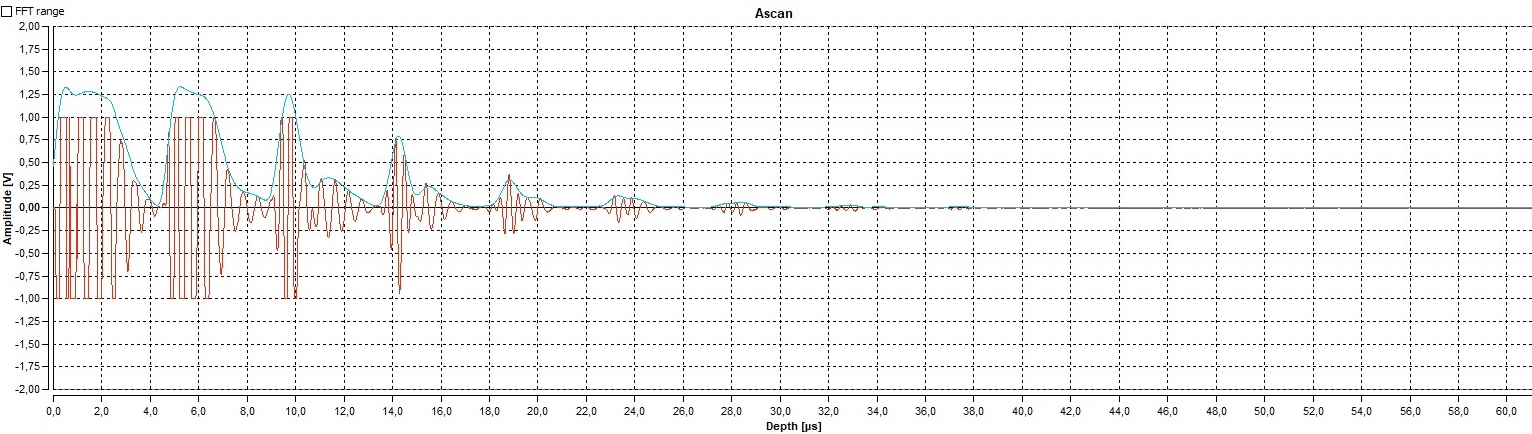
\includegraphics[width = \textwidth]{data/Geräteeinstellungen/reflexe.png}
  \caption{Aufgenommene Grafik zu den vier Reflexen.}
  \label{fig:schwingungen}
\end{figure}

Die theoretische Periodenlänge ergibt sich über die eingestellte Frequenz von $\SI{2}{\mega\hertz}$ zu 
\begin{align*}
  T = \frac{1}{\SI{2}{\mega\hertz}} = \SI{0,5}{\micro\second}.
\end{align*}
Die Schwingungsperioden sind aus \autoref{fig:schwingungen} ausgewertet worden. Die Ergebnisse sind aus \autoref{tab:perids} abzulesen.
Der Mittelwert der Schwingungen $\overline{S_i}$ ist ebenfalls in der Tabelle eingetragen.

\begin{figure}[H]
  \centering
  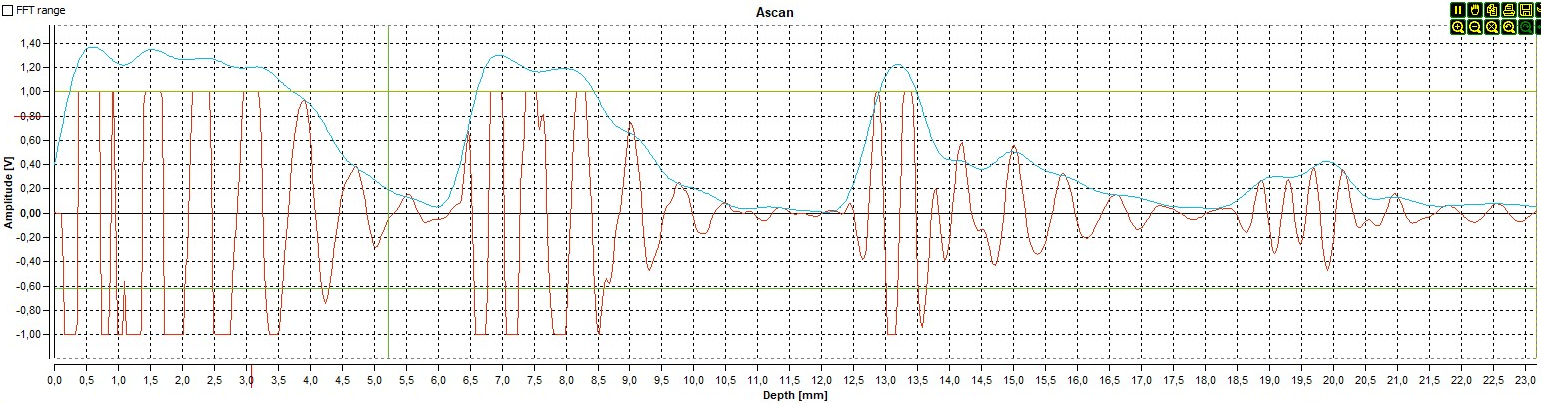
\includegraphics[width = \textwidth]{data/Geräteeinstellungen/schwingung.png}
  \caption{Aufgenommene Grafik zur Auswertung der Schwingungsperioden.}
  \label{fig:schwingungen}
\end{figure}

\begin{table}
  \centering
  \caption{Auswertung der aufgenommenen Grafik zu den Schwingungsperioden.}
  \label{tab:perids}
  \begin{tabular}{c c}
    \toprule
    Schwingung $S_i$ & Periodenlänge / $\si{\micro\second}$  \\
    \midrule
    $S_1$ & 0,50 \\
    $S_2$ & 0,54 \\
    $S_3$ & 0,58 \\
    $S_4$ & 0,54 \\
    $S_5$ & 0,57 \\
    $\overline{S_i}$ & $0.546 \pm 0.028$ \\
    \bottomrule
  \end{tabular}
\end{table}

Mithilfe des Ultraschallgerätes wird die Dicke der Acrylplatte bestimmt. Die dazu angefertigte Grafik ist in \autoref{fig:acrylplatte} dargestellt.
Der erste Peak ist die reflektierte Intensität an der Wasseroberfläche der Acrylplatte. Die Größe des zwiten Peaks beschreibt die Dicke des Acryls.
Es wird eine Tiefe von $D = \SI{6}{\milli\meter}$ bestimmt.

\begin{figure}[H]
  \centering
  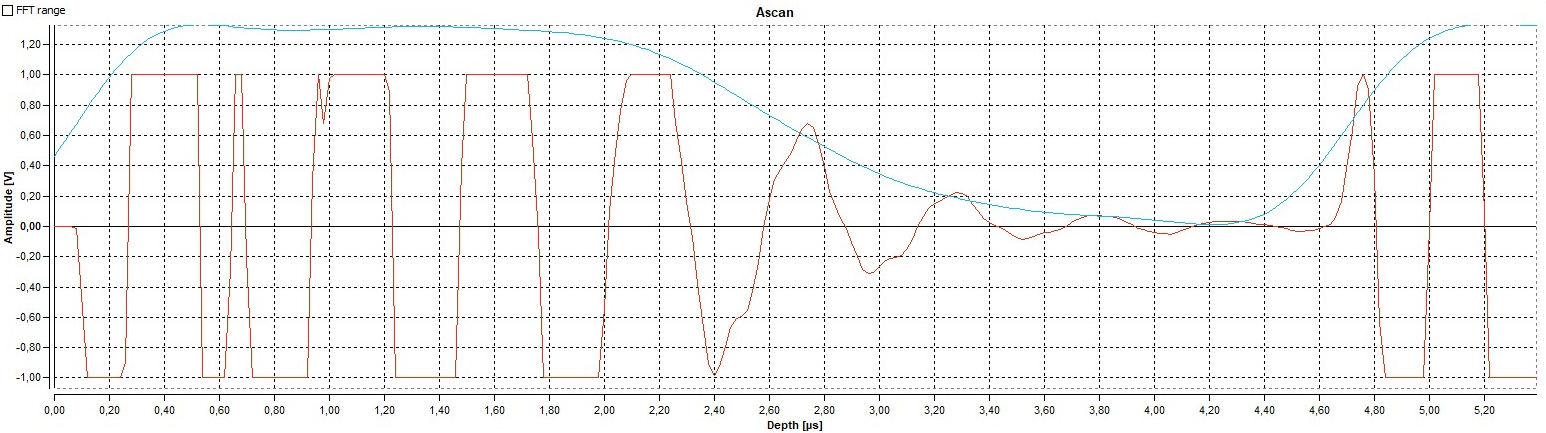
\includegraphics[width = \textwidth]{data/Geräteeinstellungen/tiefe.png}
  \caption{Aufgenommene Grafik zur Auswertung der Dicke der Acrylplatte.}
  \label{fig:acrylplatte}
\end{figure}

\subsection{Auswertung der Schallgeschwindigkeit mithilfe des Impuls-Echo-Verfahrens}
\label{subsec:schallImpEcho}

Mithilfe eines Amplituden-Scans soll nun die Laufzeit des Echos in einem Acrylzylinder ausgewertet werden. Die Lauzeiten sind in \autoref{tab:tiefeZyls} mit einem Mittelwert eingetragen.
Es wurden dabei die vier Zylinder ausgemessen. 
%Die Kombinationen sind in der Zylinderkennzeichnung markiert.
Die mit der Schieblehre ausgemessenen Längen und Durchmesser sind ebenfalls eingetragen, um sie miteinander vergleichen zu können.
Die Schallgeschwindigkeiten berechnen sich aus
\begin{align}
  s = \frac 12 \nu t \iff \nu = \frac{2s}{t}.
\end{align}
Die berechneten Schallgeschwindigkeiten $\nu$ sind ebenfalls in \autoref{tab:tiefeZyls} eingetragen

\begin{table}
  \centering
  \caption{Auswertung der aufgenommenen Grafik zu den Schwingungsperioden.}
  \label{tab:tiefeZyls}
  \begin{tabular}{c c c c c}
    \toprule
    Zylinder $Z_i$ & Länge / $\si{\milli\meter}$  &  Laufzeiten / $\si{\micro\second}$ & Durchmesser / $\si{\milli\meter}$ & $\nu_1$ / $\si{\meter\per\second\squared} $\\
    \midrule
    $Z_1$ & 40,4  & 18,32 & 40,0 & 2205,24\\
    $Z_2$ & 61,5  & 34,43 & 40,0 & 1786,23 \\
    $Z_3$ & 80,5  & 43,96 & 40,5 & 1831,21 \\
    $Z_4$ & 120,5 & 79,12 & 40,0 & 1523,01 \\
    % $Z_14$  & 160, & 32   \\
    % $Z_42$  &  &  88  \\
    % $Z_43$  &  & 74   \\
    % $Z_123$ &  & 68   \\    
    \bottomrule
  \end{tabular}
\end{table}

Der Mittelwert der Schallgeschwindigkeiten ergibt sich somit zu
\begin{align*}
  \overline \nu_1 = \SI{1.84 \pm 0,24 e3}{\meter\per\second\squared}.
\end{align*}

\subsection{Auswertung der Schallgeschwindigkeit mithilfe des Durchschallungs-Verfahrens}
\label{subsec:schallDurch}

Die Schallgeschwindigkeiten sollen nun nocheinmal mithilfe des Durchschallungsverfahren bestimmt werden.
Die mithilfe des Amplituden-Scans bestimmten Laufzeiten der jeweiligen Zylinder sind in \autoref{tab:durchZyl} eingetragen.

\begin{table}
  \centering
  \caption{Auswertung der aufgenommenen Laufzeiten.}
  \label{tab:durchZyl}
  \begin{tabular}{c c c c c}
    \toprule
    Zylinder $Z_i$ &  Laufzeiten / $\si{\micro\second}$ & $\nu_2$ / $\si{\meter\per\second\squared} $\\
    \midrule
    $Z_1$ & 30,04 & 2689.75 \\
    $Z_2$ & 43,96 & 2797.99 \\
    $Z_3$ & 59,34 & 2713.18 \\
    $Z_4$ & 88,28 & 2729.95 \\
    \bottomrule
  \end{tabular}
\end{table}

Ein Mittelwert für die Schallgeschwindigkeit beim Durchschallungs-Verfahren erfolgt somit zu
\begin{align*}
  \overline \nu_2 = \SI{2,73 \pm 0,04 e3}{\meter\per\second\squared}.
\end{align*}
